
%%%%%%%%%%%%%%%%%%%%%%% file typeinst.tex %%%%%%%%%%%%%%%%%%%%%%%%%
%
% This is the LaTeX source for the instructions to authors using
% the LaTeX document class 'llncs.cls' for contributions to
% the Lecture Notes in Computer Sciences series.
% http://www.springer.com/lncs       Springer Heidelberg 2006/05/04
%
% It may be used as a template for your own input - copy it
% to a new file with a new name and use it as the basis
% for your article.
%
% NB: the document class 'llncs' has its own and detailed documentation, see
% ftp://ftp.springer.de/data/pubftp/pub/tex/latex/llncs/latex2e/llncsdoc.pdf
%
%%%%%%%%%%%%%%%%%%%%%%%%%%%%%%%%%%%%%%%%%%%%%%%%%%%%%%%%%%%%%%%%%%%


\documentclass[runningheads,a4paper]{llncs2e/llncs}

\usepackage[T1]{fontenc}

\usepackage{amssymb,amsmath,bbm}
\setcounter{tocdepth}{3}
\usepackage{graphicx}

\usepackage{url}
\urldef{\mailjr}\path|juste.raimbault@polytechnique.edu|

  
\newcommand{\keywords}[1]{\par\addvspace\baselineskip
\noindent\keywordname\enspace\ignorespaces#1}

\newcommand{\noun}[1]{\textsc{#1}}



\begin{document}

\mainmatter  % start of an individual contribution




% first the title is needed
\title{Framing the Production of Knowledge on Complex Systems}

% a short form should be given in case it is too long for the running head
\titlerunning{A Knowledge Framework}

% the name(s) of the author(s) follow(s) next
%
% NB: Chinese authors should write their first names(s) in front of
% their surnames. This ensures that the names appear correctly in
% the running heads and the author index.
%
\author{\noun{Juste Raimbault}$^{1,2}$}
%
\authorrunning{A Knowledge Framework}
% (feature abused for this document to repeat the title also on left hand pages)

% the affiliations are given next; don't give your e-mail address
% unless you accept that it will be published
\institute{$^{1}$ UMR CNRS 8504 G{\'e}ographie-Cit{\'e}s, Paris, France\\
$^{2}$ UMR-T IFSTTAR 9403 LVMT, Champs-sur-Marne, France\\
\mailjr
}

\toctitle{Lecture Notes in Computer Science}
\tocauthor{Authors' Instructions}
\maketitle


\begin{abstract}

\keywords{Knowledge Framework, Co-evolution}
\end{abstract}



%%%%%%%%%%%%%%%%
\section{Introduction}
%%%%%%%%%%%%%%%%


The understanding of processes and conditions of scientific knowledge production are still mainly open questions, to which monuments of epistemology such as Kant's Critique of Pure Reason, and more recently Kuhn's study of ``the structure of scientific revolutions'' % TODO cit. Kuhn
or Feyerabend's advocacy for a diversity of viewpoints \cite{feyerabend1993against}, have brought elements of answer from a philosophical approach. A more empirical point of view was brought also recently with quantitative studies of science, in a way a \emph{quantitative epistemology} that goes far beyond rough bibliometric indicators % TODO cit. multidim bibliometrics
. Contributions harnessing complexity, i.e. studying complex systems in a very broad sense, can be shown to have produce very diverse frameworks that can be counted as building bricks contributing to answers to the above high-level question. % TODO define Knowledge Framework ?
 To illustrate this, we can mention frameworks in different domains, at different levels and with different purposes. For example, \cite{durantin2017disruptive} explores the potentialities of coupling engineering with design paradigms to enhance disruptive innovation. Still in Knowledge Management, using the constraint of innovation as an advantage to understand to complex nature of knowledge, \cite{carlile2004transferring} introduces knowledge domains boundaries and production processes. Also introducing a meta-framework, but in the field of system engineering, \cite{gemino2004framework} recommends to use grammars to compare Conceptual Modeling Techniques. Meta-modeling frameworks can also be understood as Knowledge Frameworks. \cite{cottineau2015modular} describes a multi-modeling framework to test hypotheses in simulation of socio-technical complex systems. \cite{golden2012modeling} postulates a unified formulation of systems, including necessarily different types of knowledge on a system on its different description components.
 
A possible explanation for this richness is the fundamental reflexive nature of the study of Complex Systems: because of the higher choice in methodology and what aspects of the system to put emphasis on, a significant part of a modeling or design entreprise is an investigation at a meta-level.  Furthermore, studies of knowledge production are mainly rooted in complexity, implying a reflexive nature of theories accounting knowledge on complexity, as Hoftenstader had well highlighted in % TODO cit Gödel Escher Bach
by noticing the importance of ``strange loops'', i.e. feedback loops allowing reflexivity such as a theory applying to itself, in what constitutes intelligence and the mind. Artificial intelligence is indeed a crucial field regarding our issues, as its progresses imply a finer understanding of the nature of knowledge. % https://arxiv.org/pdf/1704.01407.pdf TODO cit.
introduces a meta-framework for a general typology of approaches in Artificial Intelligence, what is a Knowledge Framework not in the proper sense but in a specific applied case.



The level of frameworks described above may be very general but is conditioned to a certain field or discipline, and to a certain approach or methodology. There exists to our knowledge no framework realizing a difficult exercise, that is to capture a certain structure of knowledge production at an epistemological knowledge, but conjointly is thought in a very applied perspective, with direct consequence in the design and management of complex systems. To perform that, we postulate that the tension between these two contradictory objective is an asset to avoid on one side an impossible overarching generality and on the other side a too restraining domain-specific specificity. The contribution of this paper attempts to set a basis for a Knowledge Framework realizing this in the case of Complex Systems. Based on the idea of complementary Knowledge Domains introduced by~\cite{livet2010}, its central aspect is a cognitive approach to science inducing co-evolutive processes of knowledge domains and their carriers. A first sketch of this framework was presented by~\cite{raimbault:halshs-01505084}, in the specific case of complex territorial systems as studied by theoretical and quantitative geography. We choose here an inductive approach, to show


The rest of the paper is organized as follows : 




%%%%%%%%%%%%%%%%
\section{Case Studies}
%%%%%%%%%%%%%%%%


%%%%%%%%%%%%%%%%
\subsection{Genesis of the Evolutive Urban Theory}

The first case study relates the construction of the \emph{Evolutive Urban Theory}, a geographical theory considering territorial systems from a complexity perspective, that have been developed for around 20 years. We analyse its genesis using mixed methods, namely semi-directed interviews with main contributors, and quantitative bibliometric analysis of main publications. Interviews were done following methodological standards \cite{legavre1996neutralite} to ensure a limited interference of the interviewer's experiences but not make it fully disappear to ensure a precise context enhancing the fluency of the interviewed. We use here interviews\footnote{Both length around 1h. Sound and transcript text are available under a CC Licence at \texttt{https://github.com/JusteRaimbault/Interviews}. Interviews are in French and translations here are done by the author.} with Pr. D. Pumain who introduced and developed mainly the theory, and Dr. R. Reuillon, whose research on intensive and distributed computation and model exploration has been a cornerstone of latest developments.

Let first give an overview of its content. This theory was first introduced in~\cite{pumain1997pour} which argues for a dynamical vision of city systems, in which self-organization is key. Cities are interdependent evolutive spatial entities whose interrelations produces the macroscopic behavior at the scale of city system. The city system is also described as a network of city what emphasizes its view as a complex system. Each city is itself a complex system in the spirit of~\cite{berry1964cities}, the multi-scale aspect being essential in this theory, since microscopic agents convey system evolution processus through complex feedbacks between scales. The positioning within Complex System Sciences was later confirmed~\cite{pumain2003approche}. It was shown that this theory provide an interpretation for the origin of pervasive scaling laws, resulting from the diffusion of innovation cycles between cities~\cite{pumain2006evolutionary}. The aspect of resilience of system of cities, induced by the adaptive character of these complex systems, implies that cities are drivers and adapters of social change~\cite{pumain2010theorie}. Finally, path dependance yield non-ergodicity within these systems, making ``universal'' interpretations of scaling laws difficultly compatible with evolutive urban theory~\cite{pumain2012urban}. The construction of models of urban systems has been a key component for the theory, starting with the first Simpop model~\cite{sanders1997simpop}. Later example include for example the Simpop2 model, an agent-based model taking into account economic processes, that simulates growth patterns on long time scales for Europe and the United States~\cite{doi:10.1177/0042098010377366}. The latest accomplishment of the evolutive theory relies in the output of the ERC project GeoDivercity, presented in~\cite{pumain2017urban}, that include both advanced technical (software OpenMole~\cite{reuillon2013openmole}), thematic (knowledge from SimpopLocal~\cite{schmitt2014modelisation} and Marius models~\cite{cottineau2014evolution}) and methodological (incremental modeling~\cite{cottineau2015incremental}) progresses.

The striking feature in the construction of all this is the balance between the different \emph{types} of knowledge, of which a typology will be the starting point of our construction. The relation between theoretical considerations and empirical cases studies is fundamental. Indeed, the seminal article \cite{pumain1997pour} is already positioned as an ``advocacy for a less ambitious theory, but that does not neglects the back-and-forth with observation''\footnote{p2, trad. author}. We shall now turn to interviews to better understand the implications of the intrication of types of knowledge. D. Pumain traces back germinal ideas back to her graduate student work in 1968, when ``everything started with a question of data''. The interest for cities, and \emph{change in cities}, was driven by the availability of a refined migration flow dataset at different dates. Also rapidly, ``[they] were frustrated that methods were missing'', but the access to the computation center (\emph{technical tool}) allowed the test of newly introduced methods and models, linked to the Prigogine approach to complexity. %``A presentation on entropy by Peter Allen at Creteil''
Methods were however still limited to grasp the heterogeneity of spatial interactions. A progressively specified need and a chance encounter, with ``a lady working on neural networks and agent-based modeling at the Sorbonne'', led to a bifurcation and a new level of interaction between modeling, theory and empirical knowledge: in 1997, two seminal articles, one stating the theoretical basis and the other introducing the first Simpop model, were published. From this point, it was clear that all modeling entreprise was conditioned to empirical knowledge of geographical case studies and theoretical assumptions to test. Methods and technical tools took also a necessary role, when specific model exploration methods were developed together with the Software OpenMole. R. Reuillon relates 



We back up now this qualitative analysis with a modest quantitative bibliometric analysis.






%%%%%%%%%%%%%%%%
\begin{figure}
\hspace{-4cm}
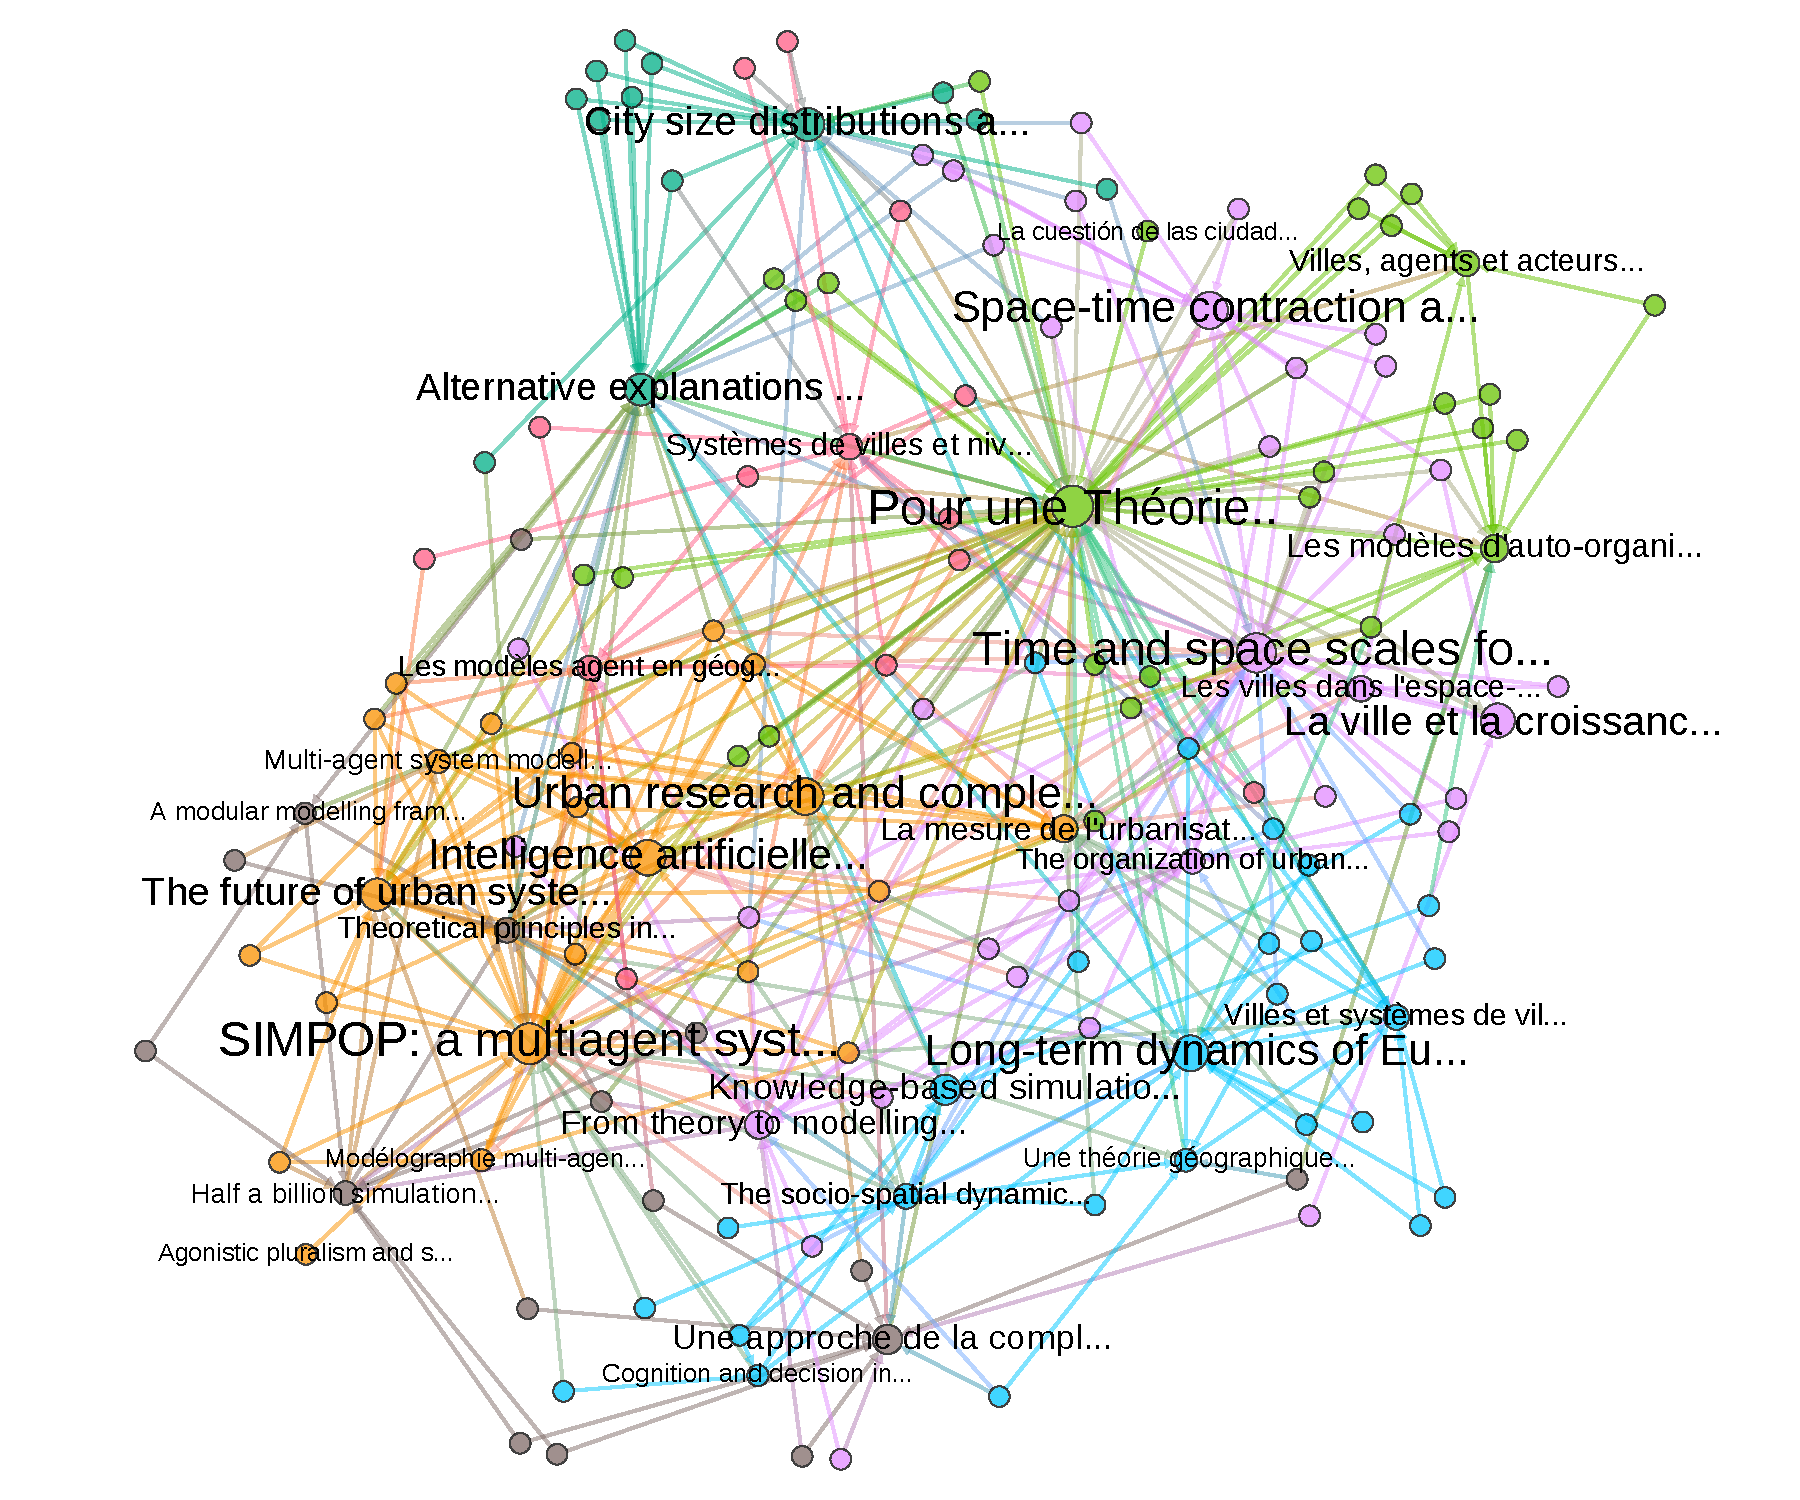
\includegraphics[width=1.5\textwidth]{figures/core}
\caption{\textbf{Citation Network of main publications of Evolutive Urban Theory.} The network is constructed the following way: starting from the two seminal publications~\cite{pumain1997pour} and \cite{sanders1997simpop}, we get citing publications, filter conditionally to one of the main contributors (\emph{Pumain}, \emph{Sanders} and \emph{Bretagnolle} being in the authors, get again citing publications and filter. It is thus a reverse citation network at depth 2. Nodes are publications, the size corresponding to eigenvector centrality, and edges are directed citation links. Colors are communities obtained with Louvain clustering algorithm (7 communities, modularity 0.379).}
\label{fig:citnw}
\end{figure}
%%%%%%%%%%%%%%%%




%%%%%%%%%%%%%%%%
\subsection{Engineering the Metropolitan}

After the glance on domains of knowledge extracted in the previous case study, we propose to take the corresponding point of view on a rather different example more related to technology and engineering


\cite{belmonte2008automatisation} automatisation de la 1 \cite{foot2005faut} portes palières
% http://cat.inist.fr/?aModele=afficheN&cpsidt=17871610
% http://cat.inist.fr/?aModele=afficheN&cpsidt=3212393 : meteor

\cite{hatchuel1988stations} innovation stations

\cite{foot1994ratp} conflits sociaux ratp

\cite{moreno2016etude} ingénierie des tunnels

\cite{balbo2016positionnement} multi-agent systems and autonomous intelligent transportation systems



%%%%%%%%%%%%%%%%
\section{Knowledge Framework}
%%%%%%%%%%%%%%%%


From the previous analyses, we can formulate know inductively the knowledge framework. As mentioned, it takes the idea of interacting domains of knowledge from the framework introduced by~\cite{livet2010}, but extends these domains and takes a novel epistemological position, focusing on co-evolutive dynamics of agents and knowledge.


\paragraph{Constraints}

To be particularly fitted for the study and management of complexity, we postulate that the framework must meet certain requirements, especially to take into account and even favor the \emph{integrative nature of knowledge}, as illustrated by the importance of interdisciplinarity and diversity in the case studies. The framework must thus be favorable to the following:
\begin{itemize}
\item Integration of disciplines, as Complex Systems are by essence at the crossing of multiple fields
\item Integration of knowledge domains, i.e. that no particular type of knowledge must be privileged in the production process\footnote{this is not incompatible with very strict system specifications, as multiple paths are possible to obtain the same fixed final state}
\item Integration of methodology types, in particular breaking the artificial boundaries between ``quantitative'' and ''qualitative'' methods, which are particularly strong in classical social sciences and humanities.
\end{itemize}


% TODO precise the central role of MODELS, as the fwk emerges in a way from their construction. closely related ot complex systems sciences, that always uses models ?


% - Epistemological fundations
% Une approche cognitive de la Science~\cite{giere2010explaining} : les \textit{agents} scientifiques~\cite{giere2010agent} à l'origine des dynamiques co-évolutives des connaissances. Cadre épistémologique du perspectivisme~\cite{giere2010scientific}.
% Compatible avec une \textit{science anarchiste} à la Feyerabend \cite{feyerabend1993against} : auto-organisation et émergence des connaissances
% 3. Extrême sur la ``check-list'' de Hacking~\cite{hacking1999social} (au delà de Kuhn) :
% - contingence maximale de par la nature dépendante au chemin du processus complexe de co-évolution des connaissances
% - degré de constructivisme maximal dans la posture perspectiviste
% - stabilité des sciences fortement couplée entre origine interne et externe de par le rôle des agents

\paragraph{Epistemological Fundations}

Our epistemological positioning relies on a cognitive approach to science, given by Giere in~\cite{giere2010explaining}. 
This approach has been shown to be operational by \cite{giere2010agent} that studies an agent-based model of science. These ideas converge with Chavalarias' Nobel Game~\cite{} % TODO cit. Nobel Game
that tests empirically the balance between exploration and falsification in the collective scientific enterprise.


\paragraph{Knowledge Domains}

We postulate the following knowledge domains :
\begin{itemize}
\item \textbf{Empirical.} Empirical knowledge of real world objects.
\item \textbf{Theoretical.} More general conceptual knowledge, implying cognitive constructions.
\item \textbf{Modeling.} Formalized \emph{medium} of the scientific perspective, rejoining Varenne's classifications of models functions~\cite{varenne2010simulations}
\item \textbf{Data.} Raw information that has been collected.
\item \textbf{Methods.} Generic structures of knowledge production.
\item \textbf{Tools.} Proto-methods and supports of others domains.
\end{itemize}

% TODO explicit why some are separated ... or in example ?


% explicit co-evolution : some domains as tools, catalysers, etc.
% DO NOT introduce morphogenesis, overcomplication for not much utility here (the notion of emerging architecture has to be deepthen)

importance of weak emergence \cite{bedau2002downward}

Holland's view on co-evolution, boundaries and niches~\cite{holland2012signals}

% - formulation
%\textbf{Definition.} La morphogenèse d'un système implique des relations circulaires causales et souvent autonomes entre les niveaux d'émergence\\ (\cite{bedau2002downward}) entre \textit{forme} et \textit{fonction} \cite{antelope2016interdisciplinary}, et exhibe dans ce sens une architecture émergente \cite{doursat2012morphogenetic}.



%\textbf{Fait stylisé.} Il existe des processus de production de connaissances scientifiques morphogénétiques, constitués d'ensemble de \textit{perspectives}, et impliquant une co-évolution des vecteurs (agents) et de domaines de connaissance (def. ci-dessous).


% \textbf{Corolaire.} La distinction entre ``quantitatif'' et ``qualitatif'' est arbitraire et sans intérêt pour la production dans ce cadre, de par la nécessité de l'ensemble de leur composantes dans l'ensemble des domaines.  

% Modèles
% Modèles de simulation
% Modèles statistiques ou mathématiques
% Modèles de données
% Modèles conceptuels



%%%%%%%%%%%%%%%%
\begin{figure}
\centering
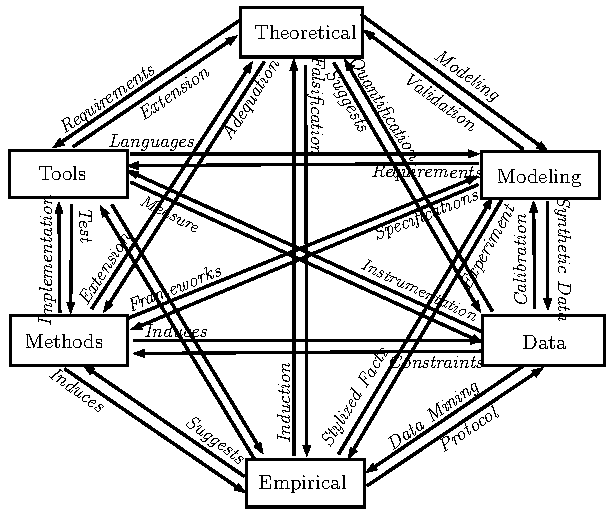
\includegraphics[width=\textwidth]{figures/framework}
\caption{\textbf{Projection of a perspective into a full network of knowledge domains}}
\label{fig:fwk}
\end{figure}
%%%%%%%%%%%%%%%%




%%%%%%%%%%%%%%%%
\section{Discussion}
%%%%%%%%%%%%%%%%



%%%%%%%%%%%%%%%%
\subsection{Application Range}

We insist that our framework does not pretend to introduce a general epistemology of scientific knowledge, but far from that is rather targeted towards reflexivity in the understanding of complex systems. The level of generality is at a very different level, but the aim to practical implication in the handling of complexity contributes to a certain genericity in applications. It is furthermore particularly suited to study Complex Systems, since more reductionist approaches can handle more compartmented production of knowledge, whereas integration of disciplines and scales and therefore domains of knowledge has been emphasized as crucial 


%%%%%%%%%%%%%%%%
\subsection{Towards a formalisation}

Our knowledge framework stays at an epistemological level, and its application must 

A perspective is defined in our case as a dataflow machine $M$ (that corresponds to the model as medium) in the sense of~\cite{golden2012modeling} that gives a convenient way to represent it and to introduce timescales and data, to which is associated an ontology $O$ in the sense of~\cite{livet2010}, i.e. a set of elements each corresponds to an entity (which can be an object, an agent, a process, etc.) of the real world. We include only two aspect (the model and the objects represented) of Giere's theory, making the assumption that purpose and producer of the perspective are indeed contained in the ontology if they make sense for studying the system.

A \emph{perspective on a system} is given by a dataflow machine $M = (i,o,\mathbb{T})$ and an associated ontology $O$. We assume that the ontology can be decomposed into atomic elements $O=(O_j)_j$.





%%%%%%%%%%%%%%%%
\section{Conclusion}
%%%%%%%%%%%%%%%%

% note : our work itself is an illustration of the fwk ?



\section*{Acknowledgments}

The author would like to thank D. Pumain and R. Reuillon for giving of their time for the interviews.



%%%%%%%%%%%%%%%%
%% Biblio
%%%%%%%%%%%%%%%%

\bibliographystyle{unsrt}
\bibliography{biblio/biblio,/Users/Juste/Documents/ComplexSystems/CityNetwork/Biblio/BibTeX/CityNetwork}





\end{document}
